\chapter{Estruturas de um Sistema RAV}
Os conceitos e definições necessárias para o desenvolvimento deste trabalho, foram apresentados nos capítulos anteriores, neste capítulo será apresentando toda a estrutura para implementação do sistema de reconhecimento de voz.

O sistema RAV proposto, foi implementado para um sistema independente do locutor, visando um jogo divertido para o maior número de pessoas possíveis, com o modo de pronúncia de palavras isoladas, e um vocabulário pequeno, que faz parte de um diciónario pré-definido. 

Este sistema foi desenvolvido em Java, com suas Apis e direcionada para sistemas operacionais Android, tendo como base a teoria dos Modelos Ocultos de Markov para o modelamento de sequencias de frames. Então cada elocução é dividida em quadros de tempos com iguais durações, extraindo seus parâmetros de cada um deles para se criar os modelos Hmms para cada palavra do dicionário, como sistemas de reconhecimento de palavras isoladas necessitam da captura do início e fim das palavras pronunciadas, o usuário deve pronunciar um comando, e depois de um breve intervalo, pronunciar o próximo, os comandos disponíveis no dicionário da aplicação são: “Direita”, “Esquerda”, “Acima” e “Abaixo”. O personagem do jogo só responderá ao comando dito, depois de reconhecer qual é o comando falado, em caso de sucesso, o jogo continua normalmente, até a vitória ou derrota do jogador, em caso do não reconhecimento da palavra, o sistema ignora a palavra dita. Outra característica importante do reconhecedor é a tentativa de capturar o humor do jogador com palavras ofensivas gravadas no dicionário, o sistema apresenta uma penalidade em caso dessas palavras serem pronunciadas.

Este trabalho pode ser dividido em 6 etapas: Aquisição da fala, Pré-Processamento, Extração de Parâmetros, Criação de referências, Classificação e Execução dos comandos.

\section{Aplicação RAV}
\begin{figure}[H]
\includegraphics[width=0.8\textwidth]{graficos/desenvolvimento_rav.eps}
\caption{Diagrama de Atividades do Sistema}
\end{figure}

Com resultado da transcrição, são definidos os comandos do jogo.

\section{Aquisição da fala}

A interação do usuário com a aplicação é feita apenas com a voz, ao iniciar o sistema, a interface de voz com usuário é habilitada, permitindo ao usuário interagir com os comandos definidos no vocabulário. Como a aplicação é destinada a dispositivos móveis, a captura do som, é feita pelo microfone do celular ou tablet, permitindo 


\section{Treinamento dos Modelos Ocultos de Markov}
A fase de treinamento é uma das etapas de maior importancia em um sistema de reconhecimento de voz independente do locutor e ser o fator determinante na obtenção de um sistema com bons resultados ou não. É o momento em que são definidos os modelos HMMs para cada palavra do vocabulário utilizado.

A definição da quantidade de estados necessários para modelar uma palavra e o número de misturas por estado não são definidos por uma regra, mas sim, dependente da familiaridade com os modelos HMMs ou por intuição, além de serem necessários muitos testes para obtenção do melhor resultado. 
%Escrever a quantidade de estados e misturas no momento da implentação

%\subsection{Aquisição do sinal de voz}


%\subsection{Pré-Processamento} 


 





